\documentclass[11pt]{article}    
\usepackage[a4paper,left=1in,right=1in,top=1in,bottom=1in]{geometry} 

\usepackage[english]{babel}
\usepackage[T1]{fontenc} 
\usepackage[utf8]{inputenc}
\usepackage{seqsplit}

\renewcommand{\familydefault}{\sfdefault} 
\usepackage{setspace}  \singlespacing  
\usepackage{graphicx}        
\usepackage[absolute]{textpos}
\usepackage{xcolor}
\usepackage{fontawesome5}
\usepackage{multirow}
\usepackage{hyperref}
\usepackage{tcolorbox}
\hypersetup{
    colorlinks,
    linkcolor={red!50!black},
    citecolor={blue!50!black},
    urlcolor={blue}
}

\definecolor{mgray}{gray}{0.85}
\definecolor{mpurple}{HTML}{68236D}
% Additional packages for the content
\usepackage{float}
\usepackage{subfig,wrapfig}
\usepackage{amsmath,amsfonts,amsthm,amssymb}
\usepackage{fancyhdr,fancybox,color}
\usepackage{enumerate}
\usepackage[amssymb]{SIunits}
\definecolor{MyBlue}{rgb}{0,0.3,0.6}
\usepackage[all]{hypcap}
\usepackage{csquotes}
\usepackage{lipsum}
\usepackage[url=false,
backend=bibtex,
style=authoryear-comp,
doi=true,
isbn=true,
backref=false,
dashed=false,
maxcitenames=2,
maxbibnames=99,
natbib=true]{biblatex}
\DeclareNameAlias{author}{family-given}
\renewbibmacro{in:}{}
\addbibresource{../_logosAndRef/references.bib}
\nonfrenchspacing

% Configurable separation between header and body
\newlength{\headertobodysep}
\setlength{\headertobodysep}{1cm}

% Header with logos and contact information
\begin{document}
\thispagestyle{empty}

% Lean header with aligned elements
\textblockorigin{0pt}{0pt}

% Durham logo on the left
\begin{textblock*}{5cm}(0.5cm,1cm)
    
\includegraphics[height=2cm]{../_logosAndRef/Durham-University.pdf}
\end{textblock*}

% Contact information in the center - vertically centered with logos
\begin{textblock*}{9cm}(6cm,1.5cm)
    \centering
    {\large \textbf{Short Title | CoMPhy Lab}}\\[0.2em]
    Department of Physics, Durham University\\[0.3em]
    \href{https://comphy-lab.org}{comphy-lab.org}
\end{textblock*}

% CoMPhy logo aligned with right margin
\begin{textblock*}{5cm}(15.5cm,1cm) % exactly 1 cm away from the right edge
    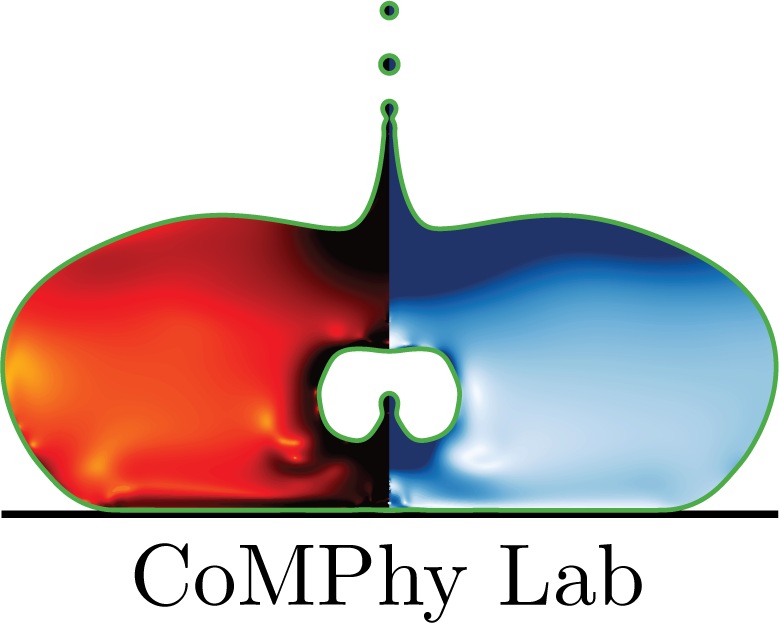
\includegraphics[height=2cm]{../_logosAndRef/CoMPhy-Lab.png}
\end{textblock*}

% Reset to normal text flow after header
\vspace*{\headertobodysep}

\begin{center}
    \begin{LARGE}
     Long Title
    \end{LARGE}
\end{center}

\noindent A few line Description

\begin{tcolorbox}[colback=mgray,colframe=mpurple,title=TL;DR]
    Too long did not read ... 
\end{tcolorbox}

\section*{Description}

\lipsum

\begin{figure}[H]
	\begin{center}
		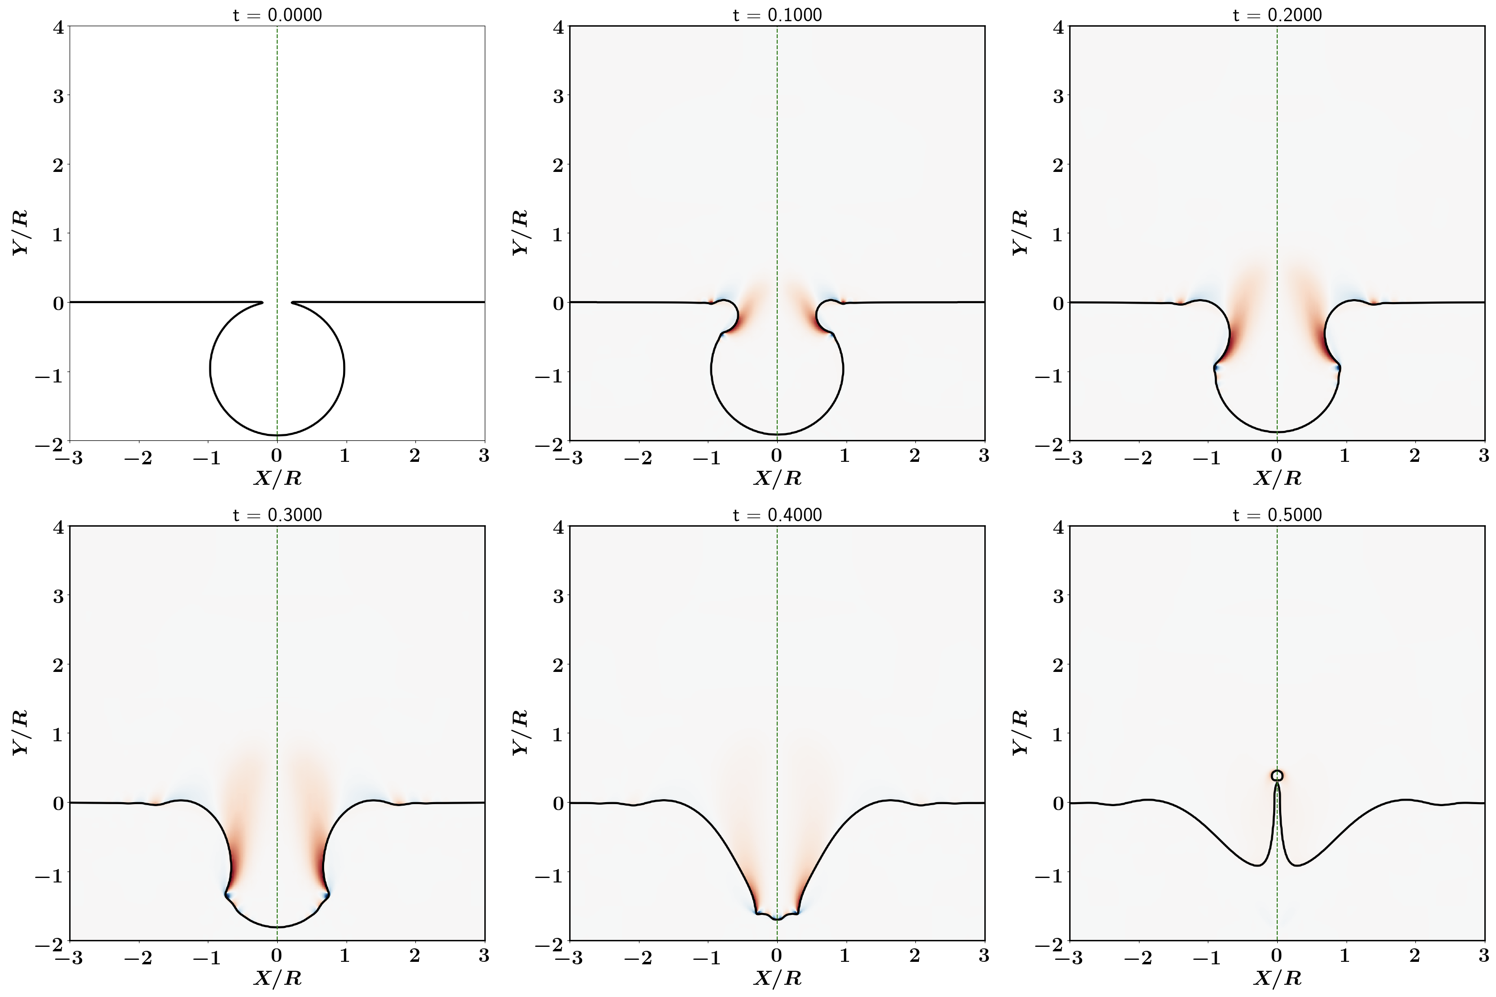
\includegraphics[width=\textwidth]{temporal.png}
		\caption{\citet{sanjay_lohse_jalaal_2021}}
		\label{fig:champange}
	\end{center}
\end{figure}

\begin{figure}[H]
\begin{center}
 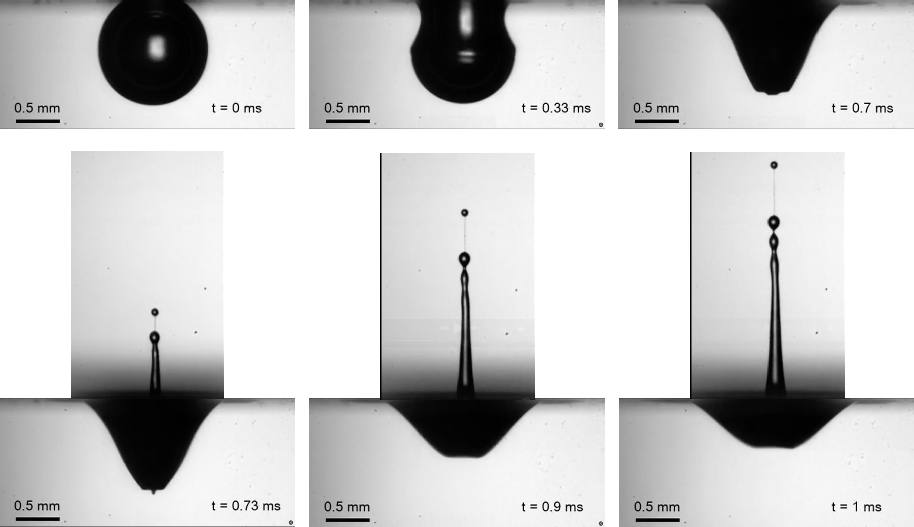
\includegraphics[width=0.95\textwidth]{schematic.pdf}
 \caption{Observation of the time evolution of the open bubble cavity. The lower rows display two views: the top view is above the water surface, while the bottom view is below the surface. }
 \label{Figure::Waves}
\end{center}
\end{figure}

\section*{What you will do and what you will learn?}

\begin{enumerate}
\item ...
\end{enumerate}

If you have any questions, feel free to contact us \href{mailto:vatsal.sanjay@comphy-lab.org}{vatsal.sanjay@comphy-lab.org}/\href{mailto:vatsal.sanjay@durham.ac.uk}{vatsal.sanjay@durham.ac.uk} or drop by Ph255 at the Department of Physics at Durham University.

\vspace*{\headertobodysep}

\noindent\textit{Last updated: \today}

\printbibliography
\end{document}